\section{Evaluation}
\label{res_overview}
 
\begin{table*}
\centering
\caption{Evaluation results overview. We evaluate two versions of mbedTLS and five
versions of OpenSSL\@. CF represents secret-dependent control-flow transfers and
DF represents secret-dependent data-flow transfers. Side-channel leakagas can
be found by symbolic execution and we run Monte Carlo to estimate the amount 
of leakage information. A summary of all vulnerabilities with the amount of
leak information can be found in the appendix.
}\label{fig:Testtt}
\begin{tabular}{clrrrrrrr}
\hline
\textbf{Algorithm} & \textbf{Implementation} & \textbf{Lekage Sites} & \textbf{CF} & \textbf{DF}
& \textbf{\# Instructions} & \textbf{Max Leakeage} & \textbf{Sym.\ Exe.} & \textbf{Monte Carlo}\\\hline
&&&&&& bits & ms & ms\\\cline{7-9}
AES & mbed TLS 2.5   & 68 & 0 & 68 & 39,855 & 8 & 570 ~~&   850 ~~\\
AES & mbed TLS 2.15  & 68 & 0 & 68 & 39,855 & 8 & 550 ~~&   829 ~~\\
AES & openssl 0.9.7  & 75 & 0 & 75 & 1,704 & 10 & 319 ~~& 7,720 ~~\\
AES & openssl 1.0.2f & 88 & 0 & 88 & 1,350 & 12 &  72 ~~& 1,500 ~~\\
AES & openssl 1.0.2k & 88 & 0 & 88 & 1,350 & 11 &  83 ~~& 1,441 ~~\\
AES & openssl 1.1.0f & 88 & 0 & 88 & 1,420 & 12 &  87 ~~& 1,454 ~~\\
AES & openssl 1.1.1  & 88 & 0 & 88 & 1,586 & 8 &   91 ~~& 1,250 ~~\\
DES & mbed TLS 2.5   & 15 & 0 & 15 & 4,596 & 1 &  114 ~~&   144 ~~\\
DES & mbed TLS 2.15  & 15 & 0 & 15 & 4,596 & 1 &  106 ~~&   137 ~~\\
DES & openssl 0.9.7  & 6 & 0 & 6 & 2,976 & 7 & 149 ~~& 4,193       ~~\\
DES & openssl 1.0.2f & 8 & 0 & 8 & 2,593 & 9 & 239 ~~& 5,311       ~~\\
DES & openssl 1.0.2k & 8 & 0 & 8 & 2,593 & 9 & 235 ~~& 5,080        ~~\\
DES & openssl 1.1.0f & 8 & 0 & 8 & 4,260 & 9 & 256 ~~& 5,027        ~~\\
DES & openssl 1.1.1  & 6 & 0 & 6 & 8,272 & 7 & 235 ~~& 4,584       ~~\\
&&&&&&& minutes & minutes\\\cline{8-9}
RSA & mbed TLS 2.5   & 6 & 6 & 0 & 22,109,246 & 9      & 38 ~~& 20  ~~\\
RSA & mbed TLS 2.15  & 12 & 0 & 12 & 24,484,441 & 9    & 39 ~~& 241  ~~\\
RSA & openssl 0.9.7  & 105 & 103 & 2 & 16,980,109 & 13 & 28 ~~& 266 ~~\\
RSA & openssl 1.0.2f & 38 & 27 & 11 & 14,468,307 & 10  & 28 ~~& 160  ~~\\
RSA & openssl 1.0.2k & 36 & 27 & 9 & 15,285,210 & 12   & 39 ~~& 282   ~~\\
RSA & openssl 1.1.0f & 31 & 22 & 9 & 16,390,750 & 13   & 32 ~~& 262 ~~\\
RSA & openssl 1.1.1  & 26 & 20 & 6 & 18,207,020 & 12   &  7 ~~& 455 ~~\\\hline
Total &              & 883 &205& 678& 128,042,089&     & 213m    ~~& 1,688m ~~\\\hline
\end{tabular}
\end{table*}

We evaluate \tool{} with the real-world crypto libraries and non-crypto libraries. 
For crypto libraries, we choose OpenSSL, mbedTLS and NaCl. 
OpenSSL and mbedTLS are the two most commonly used
crypto libraries in today's software. NaCl (pronounced "salt") is a 
new software library for encryption, decryption and signatures, etc.
NaCl is designed to have no data flow from secrets to load address and no data 
flow from secrets to branch conditions. Therefore, NaCl should have no leakage
under our attack model. 

We build the source code into 32-bit x86 Linux executables with the 
GCC 8.0 on Ubuntu 14.04. Although we use use symbol information to track
back leakage sites in the source code, our tool can
work on stripped binaries as well. We use Intel Pin version 3.7 
to record the execution trace. We run our experiments on a 2.90GHz
Intel Xeon(R) E5-2690 CPU with 128GB RAM memory.
During our evaluation process, we are interested in the following two
aspects:
\begin{enumerate}
    \item  Is \tool{} effective to detect side-channels in real-world
    crypto systems?
    \item  Can \tool{} precisely
    report the number of leaked bits in open source libraries?
    \item  Recent work has reported a number
    of side-channel vulnerabilities in open source libraries. 
    Is the number of leaked bits reported by \tool{} useful to justify 
    the sensitive level of side-channel vulnerabilities?
   
\end{enumerate}

\subsection{Evaluation Result Overview}
In this section, we present an overview of the evaluation result. 
\tool{} find 883 leakages in total from real-world crypto system libraries.
Among those 883 leak points, 205 of them are leaked due
to secret-dependent control-flow transfers and 678 of them are leaked 
due to secret-dependent memory accesses. 

For crypto libraries, \tool{} finds that secret-dependent memory accesses 
cause most leakages. 
\tool{} also identifies that most side-channel vulnerabilities 
leak very little information in practice, which confirms our initial
assumptions. 
However, we do find some sensitive leakages. 
Some of them have been confirmed by existing research that those 
vulnerabilities can be exploited to realize real attacks. 

All the symmetric key implementations in OpenSSL and mbedTLS all yield
significant leakages due to the implementation of the lookup table
to speed up the computation. Every leakages found during the evaluation
belongs to the type of secret-dependent memory accesses. We believe that
the secret-dependent control-flow transfers have been widely studied in
the past few years, and developers have patched most of those leakages. 
One method to address the leakage is to use bit-slicing. We will analyse
the corresponding countermeasure in the following sections.

\tool{} find several leakage sites for both the implementation of DES and AES
in OpenSSL and mbedTLS. \tool{} confirm that all those leakages come from
table lookups implementations. mbedTLS 2.15 and 2.5 have the same implementations
of DES and AES so they have the same leakage report. One proper fix would be 
a scalar bit-sliced implementations. However, we do not see the bit-sliced 
implementation of AES and DES in various versions of OpenSSL and mbedTLS.  
However, we find the new implementation of OpenSSL instead use typical four 1K
tables. It only uses 1K of tables. This implementation is rather easy but is
still vulnerable to a side channel attack. However, the countermeasures do
somehow decrease the total amount of leaked information.

We also evaluates our tool on the RSA implementation. With the optimizations
introduced in the paper, we do not apply any domain knowledge to 
simplify the analysis. Therefore, our tools can identify all the leakage 
sites reported by CacheD~\cite{203878} in a shorter time. Our tool
also finds that most leakages in RSA are caused in the big number implementation.
We also find newer version of RSA in OpenSSL tend to have fewer leakages detected
by \tool{}. We will discuss the version changes and corresponding leakages 
in the next section.

In addition to identifying side-channel leakages, \tool{} can also estimate how
much information is leaked from each vulnerabilities. \tool{} achieve 
the goal by estimating number of keys that satisfy the constraints.
During the Evaluation, for each leakage site, 
\tool{} will stop once 1) have 95\% confidence 
possibility that the error of estimated leaked information is less than
1 bit. 2) can not reach the termination condition after 10 minutes. In 
the case, it means the satisfying keys is very small and the leakage is 
very serious. The tools mark the Monte Carlo is failed. During the 
evaluation, we find \tool{} can quantify every side-channels leakages 
for every symmetric encryptions. For asymmetric encryptions, Monte 
Carlo quantification sometimes fail. We manually check those leakages
sites and think most of them are serious.

\subsection{Case Study of vulnerabilities}
\subsubsection{AES in mbedTLS} 
During our evaluation, we find mbedTLS 2.5 and 2.15.1 have
the same implementation of AES. Our tool provide the same leakage report
for both versions. \tool{} identify that most leakages are in 
function \emph{mbedtls\_internal\_aes\_decrypt}. (Other leakage sites are
in function \emph{mbedtls\_aes\_setkey\_enc}.) All leakages
are caused by secret-dependent memory accesses. 
Shown in the figure~\ref{mbedtls_aes}, there are seven leakage sites in 
total. Leakage 1, 2, 3 are the same and leakage 4, 5, 6, 7 are the 
same. They both use a pre-computed lookup tables to speed up computation.
However, \tool{} report Leakage 1, 2, 3 typically leak more information compared
to leakage 4, 5, 6, 7. We check the source code and find leakage 1, 2, 3 
use secret to access the lookup table \emph{RT0, RT1, RT2, RT3}, which
is 8K. On the contrary, leakage 4, 5, 6, 7 access a smaller lookup tables (2K).
Therefore, leakage 4, 5, 6, 7 leaks less information.
\begin{figure}[h!]
    \centering
\begin{lstlisting}[xleftmargin=.02\textwidth,xrightmargin=.01\textwidth]
int mbedtls_internal_aes_encrypt( mbedtls_aes_context *ctx,
const unsigned char input[16],
unsigned char output[16] )
{
uint32_t *RK, X0, X1, X2, X3, Y0, Y1, Y2, Y3;
...
for( i = ( ctx->nr >> 1 ) - 1; i > 0; i-- )
{
    AES_FROUND( Y0, Y1, Y2, Y3, X0, X1, X2, X3 ); // Leakage 1
    AES_FROUND( X0, X1, X2, X3, Y0, Y1, Y2, Y3 ); // Leakage 2
}

AES_FROUND( Y0, Y1, Y2, Y3, X0, X1, X2, X3 );     // Leakage 3

X0 = *RK++ ^ \                                    // Leakage 4
    ( (uint32_t) FSb[ ( Y0       ) & 0xFF ]       ) ^
    ( (uint32_t) FSb[ ( Y1 >>  8 ) & 0xFF ] <<  8 ) ^
    ( (uint32_t) FSb[ ( Y2 >> 16 ) & 0xFF ] << 16 ) ^
    ( (uint32_t) FSb[ ( Y3 >> 24 ) & 0xFF ] << 24 );

// X1, X2, X3 do the same computation as X0
...                                           // Leakage 5,6,7

PUT_UINT32_LE( X0, output,  0 );
...
return( 0 );
}
\end{lstlisting}
\caption{mbedtls\_internal\_aes\_encrypt}
\label{mbedtls_aes}
\end{figure}

\subsubsection{RSA in mbedTLS}
\tool{} identify several side-channel leakages for the RSA implementation
in MbedTLS. Here we introduce and analyze two cases. 

\begin{figure}[h!]
    \centering
\begin{lstlisting}[xleftmargin=.02\textwidth,xrightmargin=.01\textwidth]
...
if( mbedtls_mpi_cmp_int( N, 0 ) < 0 || ( N->p[0] & 1 ) == 0 )
    return( MBEDTLS_ERR_MPI_BAD_INPUT_DATA );
...
\end{lstlisting}
\caption{mbedtls\_mpi\_exp\_mod}
\label{mbedtls_rsa_1}
\end{figure}


\begin{figure}[h!]
    \centering
\begin{lstlisting}[xleftmargin=.02\textwidth,xrightmargin=.01\textwidth]
...
do {
    *d += c; c = ( *d < c ); d++;
}
while( c != 0 );
...
\end{lstlisting}
\caption{mpi\_mul\_hlp}
\label{mbedtls_rsa_2}
\end{figure}

\subsection{Case Study of RSA in OpenSSL}
\begin{figure*}
    \centering
    \subfloat[RSA OpenSSL 0.9.7]{
        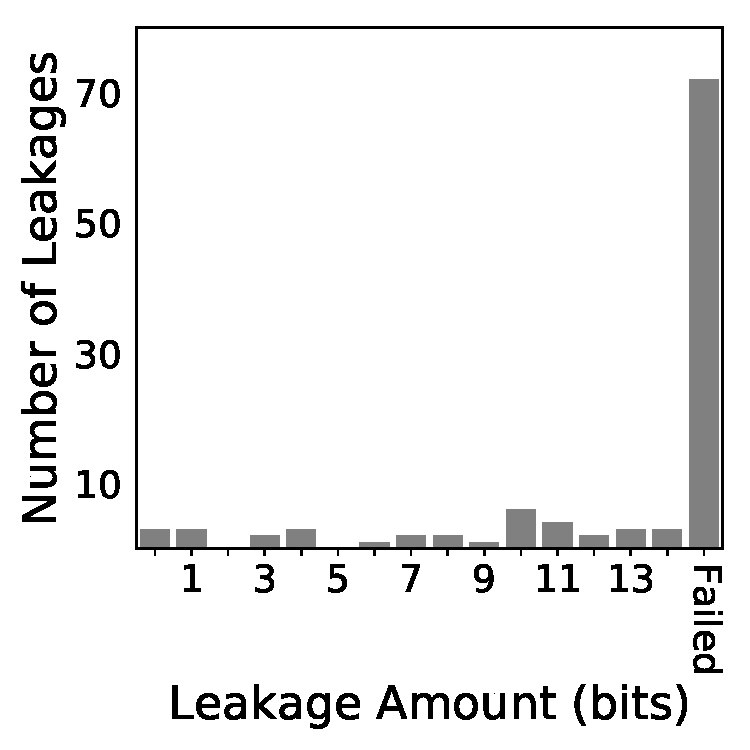
\includegraphics[width=.17\linewidth]{./figures/result/RSA-openssl-0-9-7.pdf}
    \label{fig:1}
    }
    \subfloat[RSA OpenSSL 1.0.2f]{
        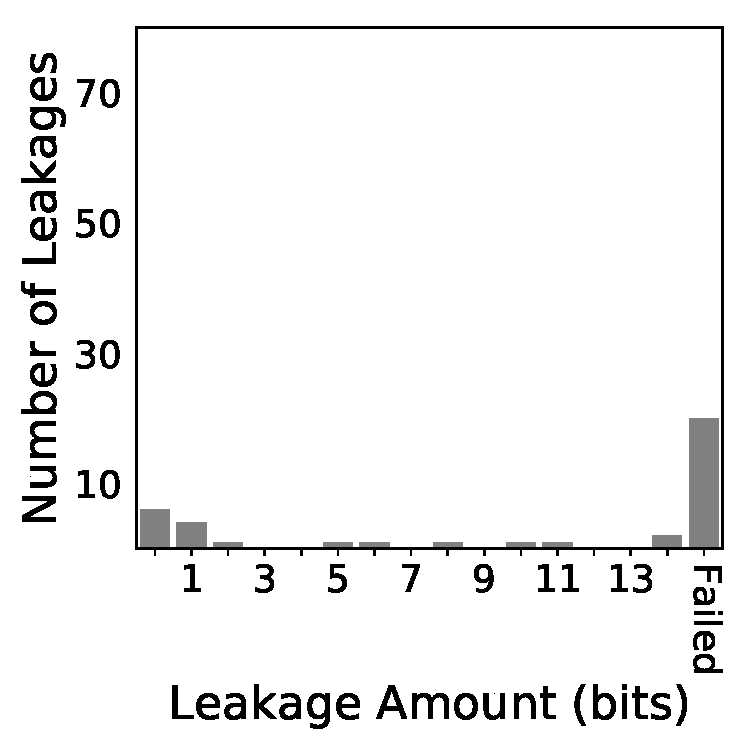
\includegraphics[width=.17\linewidth]{./figures/result/RSA-openssl-1-0-2f.pdf}
    \label{fig:1}
    }
    \subfloat[RSA OpenSSL 1.0.2k]{
        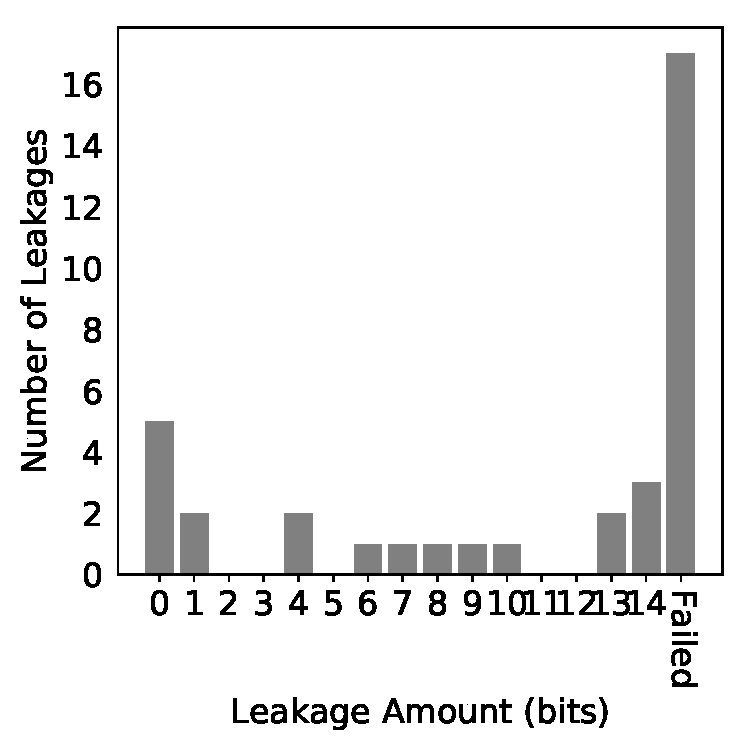
\includegraphics[width=.17\linewidth]{./figures/result/RSA-openssl-1-0-2k.pdf}
    \label{fig:1}
    }
    \subfloat[RSA OpenSSL 1.1.0f]{
        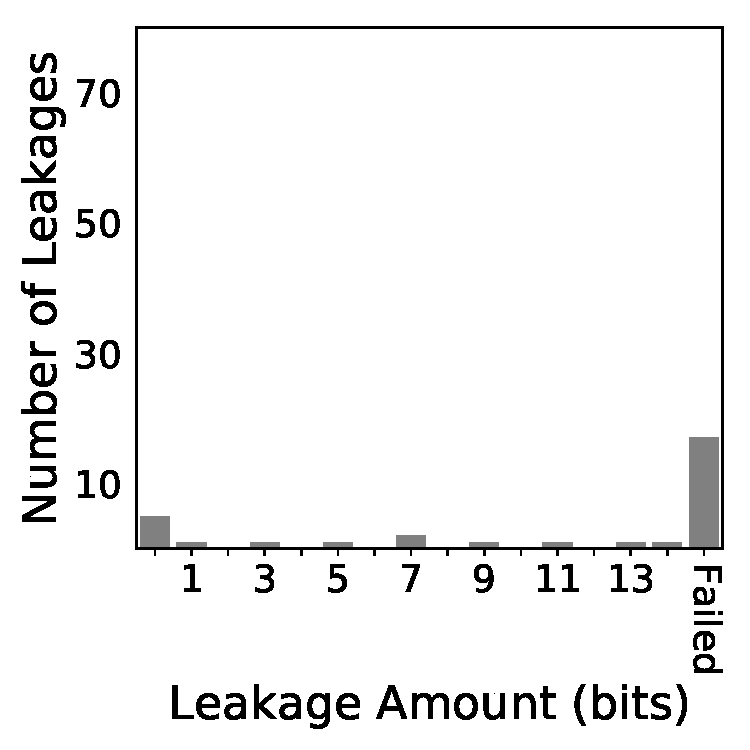
\includegraphics[width=.17\linewidth]{./figures/result/RSA-openssl-1-1-0f.pdf}
    \label{fig:1}
    }
    \subfloat[RSA OpenSSL 1.1.1]{
        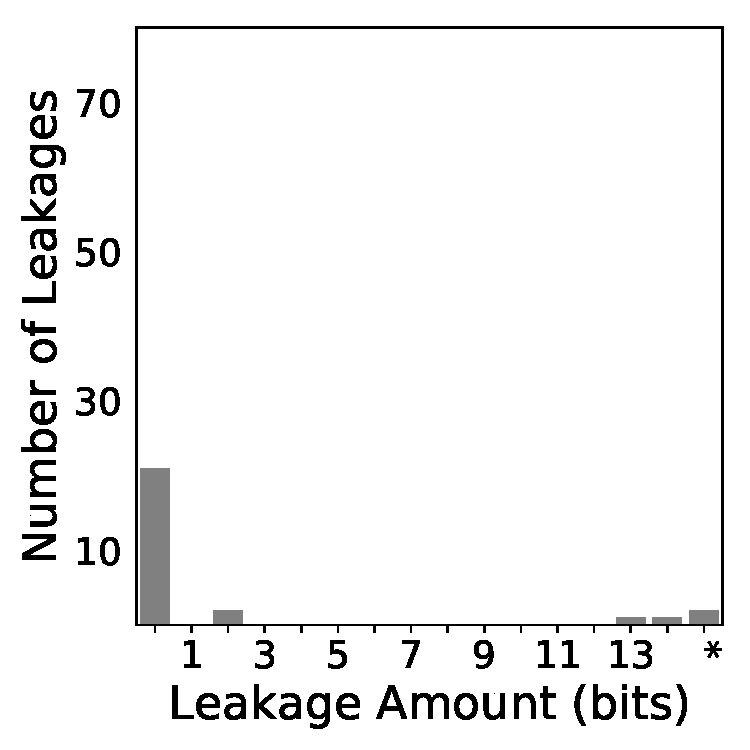
\includegraphics[width=.17\linewidth]{./figures/result/RSA-openssl-1-1-1.pdf}
    \label{fig:1}
    }
\caption{RSA implementation in different versions of OpenSSL}
For crypto libraries, it is likely that a newer version has less vulnerabilities
compared to the previous version.
\end{figure*}
\subsection{Analysis of Software Countermeasures}
\subsubsection{Bit-slicing}
\subsubsection{Scatter and Gather}
\subsubsection{Smaller Lookup Tables}
